\chapter{Neutrino Oscillation Physics}
\label{chap:NeutrinoOscillationPhysics}
Neutrino Oscillation Physics Chapter

\section{Discovery of Neutrinos}
\label{sec:NeutrinoOscillationPhysics_Discovery}

At the start of the \quickmath{20^{th}} century, the electrons emitted from \quickmath{\beta}-decay of the nucleus were found to have a continuous energy spectrum \cite{Chadwick:262756, Ellis1927-qf}. This observation seemingly broke the conservation of energy invoked within the nuclear models of that period.  Postulated in 1930 by Pauli as the solution to this problem, the neutrino (originally termed ``neutron'') was theorised to be an electrically neutral spin-\quickmath{1/2} fermion with a mass on the same order of magnitude as the electron \cite{Pauli:1930pc}. This particle was to be emitted with the electron in \quickmath{\beta}-decay to ellivate the apparent breaking of energy conservation. As a predecessor of weak interaction model, Fermi's theory of \quickmath{\beta}-decay developed the understanding by coupleing the four consistuent particles; electron, proton, neutron and neutrino, into a consistent model \cite{Fermi:1934hr}.

Whilst Pauli was not convinced of the ability to detect neutrinos, the first observations of the particle were made in mid-1950s by using inverse \quickmath{\beta}-decay (IBD) process, \quickmath{\bar{\nu}_{e} + p \rightarrow n + e^{+}}, from neutrinos generated by nuclear reactors \cite{reines_cowan_1,reines_cowan_2}.
%The detector consisted of cadium-doped water targets surronded by liquid scintillator, which was monitored by a suite of photo-multiplier tubes.
The detector consisted of two parts; a neutrino interaction medium and a liquid scintialltor. The interaction medium is built from two water tanks, each loaded with cadium chloride to allow increased efficiency of neutron capture. The positron emitted from IBD annihaltes, \quickmath{e^{+} + e^{-} \rightarrow 2\gamma}, generating a prompt signal, whereas the neutron is captured on the cadmium via \quickmath{n + ^{108}Cd \rightarrow ^{109m}Cd \rightarrow ^{109}Cd + \gamma}, producing a delayed signal. The experiment also observed an increase in the neutrino event rate when the reactor was operating compared to when it was switched off, in much the same way as modern reactor neutrino experiments operate.

After the discovery of the \quickmath{\nu_{e}}, the natural question of how many flavours of neutrino exist and how that aligns with the number of charged leptons was asked. In 1962, a measurement of the \quickmath{\nu_{\mu}} was conducted at the Brookhaven National Laboratory \cite{Lederman}. A proton beam was directed at a beryllium target, generating a \quickmath{\pi} dominated beam which then decayed via \quickmath{\pi^{+} \rightarrow \mu^{+} + \nu_{\mu}} and the subsequent interactions of the \quickmath{\nu_{\mu}} were observed. The final observation to be made was that of the \quickmath{\nu_{\tau}} from the DONUT experiment \cite{tau_nu_disc}.

\section{Theory of Neutrino Oscillation}
\label{sec:NeutrinoOscillationPhysics_EvidenceForNeutrinoOscillation}

As direct evidence of beyond Standard Model physics, a neutrino generated with lepton flavour \quickmath{\alpha} can mutate into a different lepton flavour \quickmath{\beta} after propagating some distance. This phenomena is called neutrino oscillation and requires that neutrinos must have a non-zero mass. This behaviour has been characterised by the Pontecorvo-Maki-Nakagawa-Sakata (PMNS) \cite{p1,p2,km} mixing matrix which describes how the flavour and mass eigenstates are associated. This is analogous to the Cabbibo-Kobayashi-Maskawa (CKM) \cite{cabbibo} matrix found in quark physics.

\subsection{Three Flavour Oscillations}
\label{sec:NeutrinoOscillationPhysics_3FlavourOsc}

The PMNS parameterisation defines three flavour eigenstates, \quickmath{\nu_{e}}, \quickmath{\nu_{\mu}} and \quickmath{\nu_{\tau}} (denoted \quickmath{\nu_{\alpha}}), which are assigned based upon the weak interaction flavour states, and three mass eigenstates, \quickmath{\nu_{1}}, \quickmath{\nu_{2}} and \quickmath{\nu_{3}} (denoted \quickmath{\nu_{i}}). Each mass eigenstate is the superposition of all three flavour states,

\begin{equation}
  \label{eq:NeutrinoOscillationPhysics_Superposition}
  \left|\nu_{i}\right> = \sum_{\alpha}\mathrm{U}_{\alpha i}\left|\nu_{\alpha}\right>.
\end{equation}

\quickmath{\mathrm{U}} is the PMNS matrix which correlates the mass and flavour eigenstates

\begin{equation}
  \label{eq:NeutrinoOscillationPhysics_PMNSReduced}
  \mathrm{U} = \begin{pmatrix} \mathrm{U}_{e1} & \mathrm{U}_{e2} & \mathrm{U}_{e3} \\ \mathrm{U}_{\mu 1} & \mathrm{U}_{\mu 2} & \mathrm{U}_{\mu 3} \\ \mathrm{U}_{\tau 1} & \mathrm{U}_{\tau 2} & \mathrm{U}_{\tau 3} \end{pmatrix}.
\end{equation}

The propogation of a neutrino through space is determined by the superposition of the three mass eigenstates. Therefore, the propogation of a neutrino flavour eigenstate can be re-written as a plane-wave solution to the time-dependent Schr{\"o}dinger equation,

\begin{equation}
  \label{eq:NeutrinoOscillationPhysics_TimeDepSuperposition}
  \left|\nu_{\alpha}(t)\right> = \sum_{i}\mathrm{U}^{*}_{\alpha i}\left|\nu_{i}\right>e^{-i \phi_{i}}.
\end{equation}

The probability of observing a neutrino of flavour eigenstate \quickmath{\beta} from one which originated as flavour \quickmath{\alpha} can be calculated as,

\begin{equation}
  \label{eq:NeutrinoOscillationPhysics_ProbabilityComplexForm}
  P(\nu_{\alpha} \rightarrow \nu_{\beta}) = \left| \left< \nu_{\beta} | \nu_{\alpha}(t) \right> \right|^{2} = \sum_{i,j} \mathrm{U}^{*}_{\alpha i}\mathrm{U}_{\beta i}\mathrm{U}_{\alpha j}\mathrm{U}^{*}_{\beta j} e^{-i(\phi_{j}-\phi_{i})}
\end{equation}

The \quickmath{\phi_{i}} term can be expressed in terms of the energy, \quickmath{E_{i}}, and magnitude of the three momentum, \quickmath{p_{i}}, of the neutrino, \quickmath{\phi_{i} = E_{i}t - p_{i}x}. Therefore,

\begin{equation}
  \label{eq:NeutrinoOscillationPhysics_PhaseDifference}
  \phi_{j}-\phi_{i} = E_{j}t - E_{i}t - p_{j}x + p_{i}x .
\end{equation}

For a relativistic particle, \quickmath{E_{i} \gg m_{i}},

\begin{equation}
  p_{i} = \sqrt{E^{2}_{i} - m^{2}_{i}} \approx E_{i} - \frac{m^{2}_{i}}{2E_{i}}.
\end{equation}

Making the approximation that the neutrino mass eigenstates were created with the same energy and that \quickmath{x = t = L}, where \quickmath{L} is the distance travelled by the neutrino, \autoref{eq:NeutrinoOscillationPhysics_PhaseDifference} then becomes

\begin{equation}
  \phi_{j}-\phi_{i} = \frac{\Delta m^{2}_{ij} L}{2E},
\end{equation}

where \quickmath{\Delta m^{2}_{ij} = m^{2}_{i} - m^{2}_{j}}. This, teamed with further use of unitarity relations results in \autoref{eq:NeutrinoOscillationPhysics_ProbabilityComplexForm} becoming

\begin{equation}
  \label{eq:NeutrinoOscillationPhysics_ProbabilityComplexForm2}
  P(\nu_{\alpha} \rightarrow \nu_{\beta}) = \delta_{\alpha \beta} - 4 \sum_{i>j} \mathbb{R} \left( \mathrm{U}^{*}_{\alpha i}\mathrm{U}_{\beta i}\mathrm{U}_{\alpha j}\mathrm{U}^{*}_{\beta j} \right) \sin^{2} \left( \frac{\Delta m^{2}_{ij} L}{4E} \right) \\ + \left( - \right) 2 \sum_{i>j} \mathbb{I} \left( \mathrm{U}^{*}_{\alpha i}\mathrm{U}_{\beta i}\mathrm{U}_{\alpha j}\mathrm{U}^{*}_{\beta j} \right) \sin \left( \frac{\Delta m^{2}_{ij} L}{2E} \right) \notag.
\end{equation}

Where the negative sign is included for the oscillation probability of antineutrinos.

Typically, the PMNS matrix is parameterised into three mixing angles, a charge parity (CP) violating phase \quickmath{\delta_{CP}}, and two Majorana phases \quickmath{\alpha_{1,2}},

\begin{equation}
  \label{eq:NeutrinoOscillationPhysics_PMNS}
  \mathrm{U} =
  \underbrace{\begin{pmatrix} 1 & 0 & 0 \\ 0 & c_{23} & s_{23} \\ 0 & -s_{23} & c_{23} \end{pmatrix}}_{\text{Atmospheric, Accelerator}}
  \underbrace{\begin{pmatrix} c_{13} & 0 & s_{13}e^{-i \delta_{CP}} \\ 0 & 1 & 0 \\ -s_{13}e^{-i \delta_{CP}} & 0 & c_{13} \end{pmatrix}}_{\text{Reactor, Accelerator}}
  \underbrace{\begin{pmatrix} c_{12} & s_{12} & 0 \\ -s_{12} & c_{12} & 0 \\ 0 & 0 & 1 \end{pmatrix}}_{\text{Reactor, Solar}}
  \underbrace{\begin{pmatrix} e^{i\alpha_{1}/2} & 0 & 0 \\ 0 & e^{i\alpha_{2}/2} & 0 \\ 0 & 0 & 1 \end{pmatrix}}_{\text{Majorana}}.
\end{equation}

Where \quickmath{s_{ij} = \sin(\theta_{ij})} and \quickmath{c_{ij} = \cos(\theta_{ij})}. The mixing angles are often referred to by the style of experiment which best constrains these parameters; \quickmath{(1,2)} as ``solar'', \quickmath{(2,3)} as ``atmospheric'' and \quickmath{(1,3)} as ``reactor''. Many neutrino experiments aim to measure the PMNS parameters from a wide array of origins, as is the purpose of this thesis.

The Majorana phase containing matrix included within \autoref{eq:NeutrinoOscillationPhysics_PMNS} is only included for completeness. For the purposes of an oscillation analysis experiment, any term in this oscillation probability calculation containing this phase disappears due to taking the expectation value of the PMNS matrix.

A two flavour approximation can be attained when one assumes the third mass eigenstate is degenerate with another. As discussed in \autoref{sec:NeutrinoOscillationPhysics_OscillationMeasurements}, it is found that \quickmath{\Delta m^{2}_{21} \ll |\Delta m^{2}_{31}|} such that this two flavour approximation is reasonable for understanding the features of the oscillation. In this two flavour case, the mixing matrix becomes

\begin{equation}
  \label{eq:NeutrinoOscillationPhysics_PMNS_2Flavour}
  \mathrm{U_{\text{2 Flav.}}} = \begin{pmatrix} \cos(\theta) & \sin(\theta) \\ -\sin(\theta) & \cos(\theta) \end{pmatrix}
\end{equation}

which culminates in the oscillation proabability,

\begin{equation}
  \label{eq:NeutrinoOscillationPhysics_PMNS_2FlavourOscProb}
  P(\nu_{\alpha} \rightarrow \nu_{\beta}) = \delta_{\alpha \beta} - \left( + \right) \sin^{2} \left( 2\theta \right) \sin^2 \left( \frac{\Delta m^{2} L}{4E} \right).
\end{equation}

The oscillation probability is a sinusodial function depending upon the distance over which the neutrino propagates. The frequency and amplitude of oscillation is dependent upon the ratio of the \quickmath{\Delta m^{2} / 4E} and \quickmath{\sin^2{2\theta}}, respectively. For more human-readable units, the maximum oscillation probability for a fixed value of \quickmath{\theta} is given at \quickmath{L[km]/E[GeV] \sim 1.27 / \Delta m^{2}}. It is this calculation that determines the best \quickmath{L/E} value for a given experiment to be designed around for measurements of a specific value of \quickmath{\Delta m^{2}}.

\subsection{The MSW Effect}
\label{sec:NeutrinoOscillationPhysics_MSW}

\autoref{sec:NeutrinoOscillationPhysics_3FlavourOsc} describes the theory of neutrino oscillation in a vacuum but beam neutrinos and atmospheric neutrinos originating from below the horizon propagate through matter in the Earth. The coherent scattering of neutrinos from a material target modifies the energy of the mass eigenstates resulting in a change to the oscillation probability. Notably, charged current scattering (\quickmath{\nu_{e} + e^{-} \rightarrow \nu_{e} + e^{-}}, propagated by a \quickmath{W} boson) only effects electron neutrinos compared to the neutral current scattering (\quickmath{\nu_{l} + l^{-} \rightarrow \nu_{l} + l^{-}}, propagated by a \quickmath{Z^{0}} boson) which does not favour any neutrino flavour. In the two-flavour limit, the effective mixing parameter becomes

\begin{equation}
  \label{eq:NeutrinoOscillationPhysics_2Flavour_MSW}
  \sin^{2}(2\theta) \rightarrow \sin^{2}(2\theta_{m}) = \frac{\sin^{2}(2\theta)}{(A/\Delta m^{2} - \cos(2\theta))^{2} + \sin^{2}(2\theta)},
\end{equation}

where \quickmath{A = 2\sqrt{2}G_{F}N_{e}E} with \quickmath{N_{e}} is the electron density of the medium and \quickmath{G_{F}} is Fermi's constant. It is clear to see that there exists a value of \quickmath{A = \Delta m^{2} \cos(2\theta)} for \quickmath{\Delta m^{2} > 0} which results in a divergent mixing parameter. This is known as the Mikheyev-Smirnov-Wolfenstein (MSW) effect (or more clloquially, the matter resonance) which regenerates the electron neutrino component of the neutrino flux \cite{Smirnov2003-yb, msw, wolfenstein}. The density at which the resonance occurs is given by

\begin{equation}
  \label{eq:NeutrinoOscillationPhysics_ResonanceDensity}
  N_{e} = \frac{\Delta m^{2} \cos(2\theta)}{2\sqrt{2} G_{F} E}
\end{equation}

At densities lower than this critical value, the oscillation probability will be be much closer to that from vacuum oscillation. As seen, the resonance occuring from the MSW effect depends on the sign of \quickmath{\Delta m^{2}}. Therefore, any neutrino oscillation experiment which obsreves neutrinos which have propagated through matter can have some sensitivity to the ordering of the neutrino mass eigenstates.

For an experiment observing atmospheric neutrinos propagating through the Earth such as the studies presented in this thesis, a model of the Earth's density and layering is required. The model used within this analysis is the Preliminary Reference Earth Model (PREM) \cite{Dziewonski1981-sp}. This model approximates the Earth as four layers of constant density as described in \autoref{tab:NeutrinoOscillationPhysics_PREMModel}. The density measurements provided in this model are provided in terms of masss density, whereas neutrino oscillations are sensitive to the electron number density. Consequently, the chemical compositon of each layer multiplied by the mass density gives the relevent value for oscillation probabilities.

\begin{table}[ht!]
    \centering
    \begin{tabular}{c|c|c|c}
      \hline
      Layer & Outer Radius [\quickmath{\text{km}}] & Density [\quickmath{\text{g/cm}^{3}}] & Chemical composition (Z/A) \\
      \hline
      Inner Core & \quickmath{1220} & \quickmath{13} & \quickmath{0.468 \pm 0.029} \\
      Outer Core & \quickmath{3480} & \quickmath{11.3} & \quickmath{0.468 \pm 0.029} \\
      Lower Mantle & \quickmath{5701} & \quickmath{5.0} & \quickmath{0.497} \\
      Transition Zone & \quickmath{6371} & \quickmath{3.3} & \quickmath{0.497} \\
      \hline
    \end{tabular}
    \caption{Description of the four layers of the Earth invoked within the PREM model \cite{Dziewonski1981-sp}.}
    \label{tab:NeutrinoOscillationPhysics_PREMModel}
\end{table}

The beam oscillation probability in this thesis uses a baseline of \quickmath{295 \text{km}} and density \quickmath{2.6 \text{g/cm}^{3}}.

\section{Neutrino Oscillation Measurements}
\label{sec:NeutrinoOscillationPhysics_OscillationMeasurements}

As evidence of beyond standard model physics, the 2015 Nobel Prize in Physics was awarded to the Super-Kamiokande (SK) and Sudbury Neutrino Observatory (SNO) collaborations for the first definitive observation of solar and atmospheric neutrino oscillation. Since then, the field has seen a wide array of oscillation measurements from a variety of neutrino sources. As seen in \autoref{sec:NeutrinoOscillationPhysics_3FlavourOsc}, the neutrino oscillation probability is dependent on the ratio of the propagation baseline, \quickmath{L}, to the neutrino energy, \quickmath{E}, which determines the flavour of neutrino oscillation a particular experiment is sensitive to.

As illustrated in \autoref{fig:NeutrinoOscillationPhysics_EnergySpectrum}, neutrino energies span a wide range of energies. The least energetic neutrinos are from diffuse supernovae and terrestrial neutrinos at \quickmath{O(1)\text{eV}} whereas the most energetic neutrinos originate from atmospheric and galactic neutrinos of \quickmath{>O(1)\text{TeV}}. 

\begin{figure}[h]
  \begin{subfigure}[t]{0.95\textwidth}
    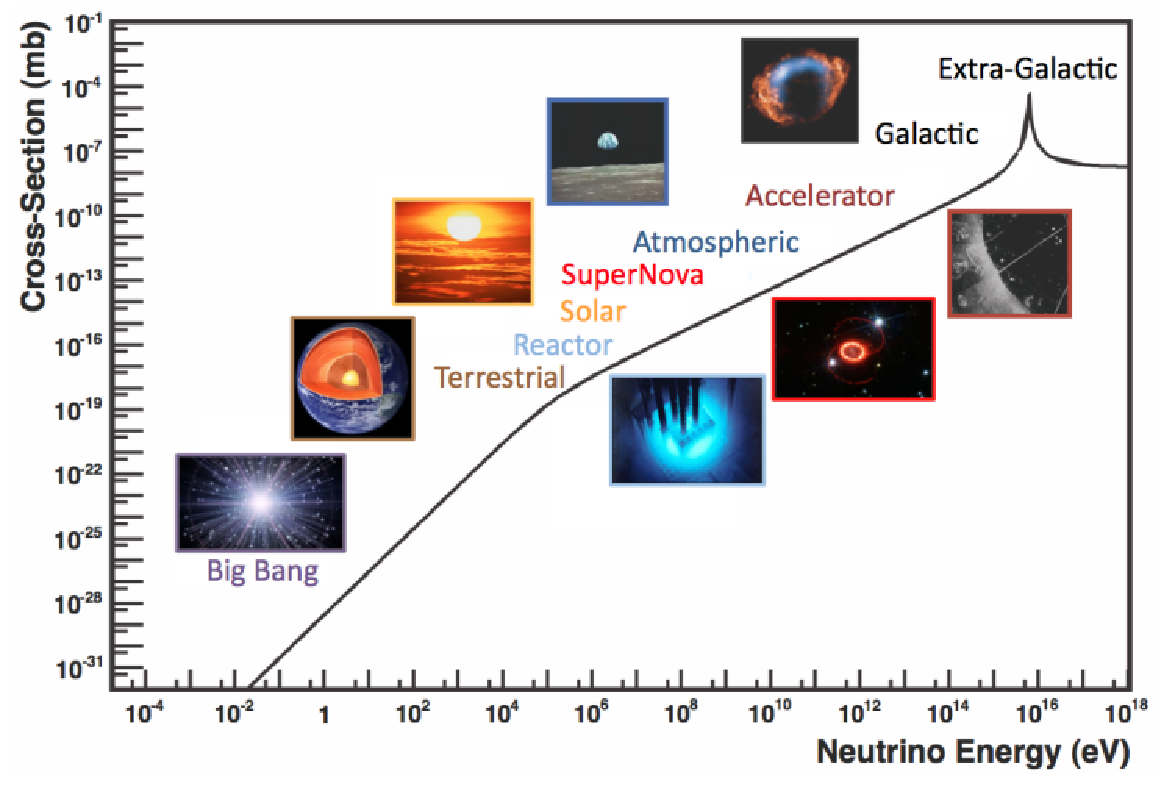
\includegraphics[width=\textwidth, trim={0mm 0mm 0mm 0mm}, clip,page=1]{Figures/Theory/EnergySpectrum.pdf}
  \end{subfigure}
  \caption{The energy spectrum of neutrinos from various natural and man-made sources. Taken from \cite{Formaggio:2012cpf}}
  \label{fig:NeutrinoOscillationPhysics_EnergySpectrum}
\end{figure}

\subsection{Solar Neutrinos}
\label{subsec:NeutrinoOscillationPhysics_SolarNeutrinos}

Solar neutrinos are emitted from interaction chains contained within the fusion reaction at the center of the Sun. The solar neutrino flux given as a function of neutrino energy for different fusion and decay chains is illustrated in \autoref{fig:NeutrinoOscillationPhysics_SolarNeutrinoFlux} (From \cite{Bellerive2004-ur}). Whilst proton-proton fusion generates the largest flux of neutrinos, the neutrinos are of low energy and are difficult to reconstruct. Consequently most experiments focus on the neutrinos from the decay of \quickmath{^{8}B} (via \quickmath{^{8}B \rightarrow ^{8}Be^{*} + e^{+} + \nu_{e}}), which are higher energy.

\begin{figure}[h]
  \begin{subfigure}[t]{0.80\textwidth}
    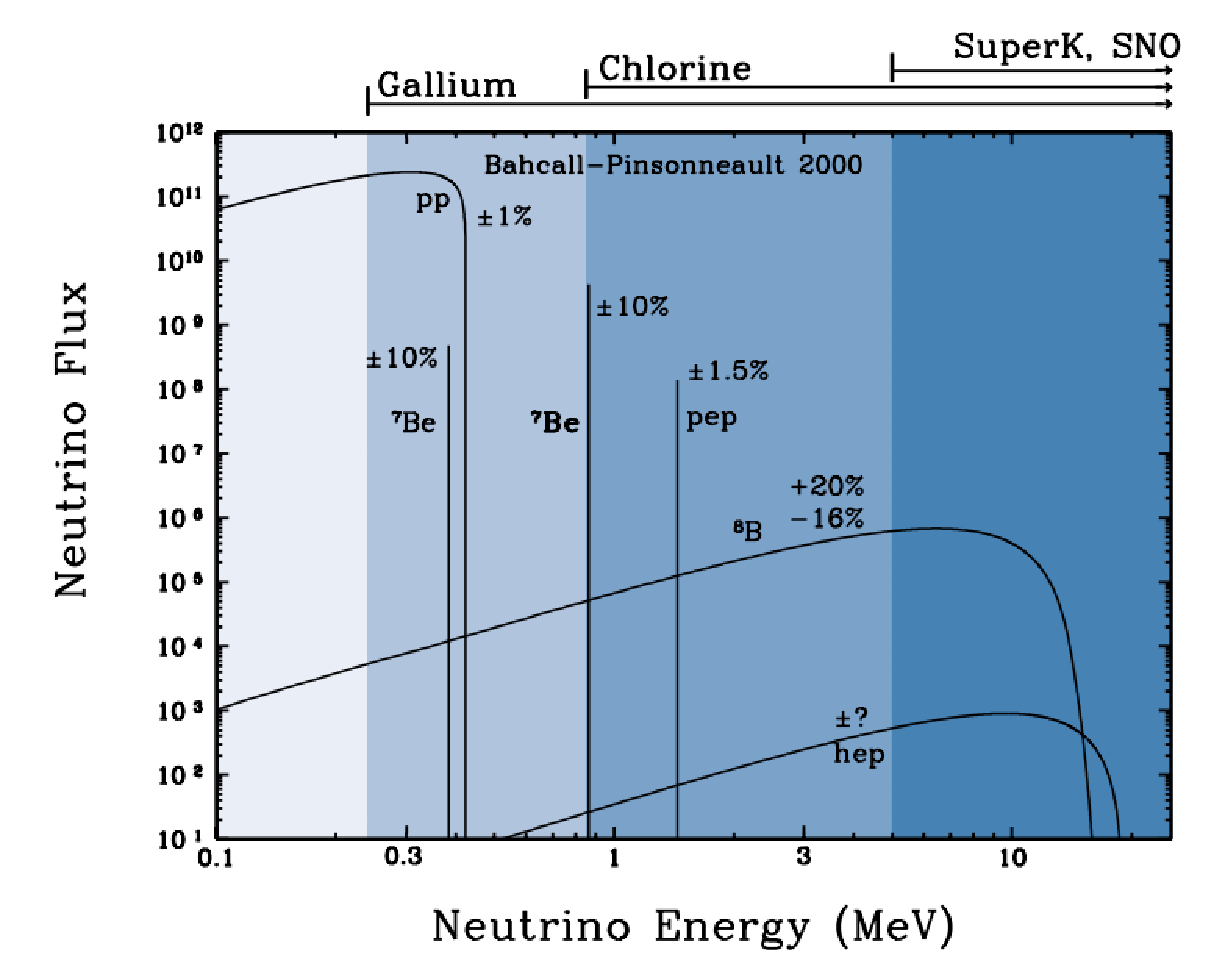
\includegraphics[width=\textwidth, trim={0mm 0mm 0mm 0mm}, clip,page=1]{Figures/Theory/SolarNeutrinoFlux.pdf}
  \end{subfigure}
  \caption{The solar neutrino flux as a function of neutrino energy for various fusion reaction and decay chains as predicted by the Standard Solar Model. Taken from \cite{Bellerive2004-ur}.}
  \label{fig:NeutrinoOscillationPhysics_SolarNeutrinoFlux}
\end{figure}

The first measurements of solar neutrinos observed a significant reduction in the event rate compared to predictions from the Standard Solar Model \cite{PhysRevLett.20.1205, Vinyoles2017-vv}. The proposed solution to this ``solar neutrino problem'' was \quickmath{\nu_{e} \leftrightarrow \nu_{\mu}} oscillations in a precursory version of the PMNS model \cite{Gribov1969-xi}. The Kamiokande \cite{PhysRevLett.63.16}, Gallex \cite{Hampel1999-of} and Sage \cite{PhysRevC.60.055801} experiments confirmed the \quickmath{\sim 0.5} deficit of solar neutrinos.

The conclusive solution to the ``solar neutrino problem'' was determined by the SNO collaboration \cite{Ahmad2002-zv}. Using a deutrium water target to observe \quickmath{^{8}B} neutrinos, the event rate of charged current (CC), neutral current (NC) and elastic scattering (ES) interactions (Given in \autoref{eq:NeutrinoOscillationPhysics_SNOInteractions}) measured. CC events can only occur for electron neutrinos, whereas the other interaction channels are agnostic to neutrino flavour (Although the ES reaction is more sensitive to electron neutrino interactions). This meant that there was a direct measurement of the \quickmath{\nu_{e}} and total neutrino flux. It was concluded that the CC and ES reaction rates were consistent with the deficit previouly observed but notably that the NC reaction rate was only consistent with the other interaction rates under the hypothesis of flavour transformation.

\begin{equation}
  \label{eq:NeutrinoOscillationPhysics_SNOInteractions}
  \begin{split}
    \nu_{e} + d &\rightarrow p + p + e^{-} \hspace{2cm} (CC) \\
    \nu_{x} + d &\rightarrow p + n + \nu_{x} \hspace{2.02cm} (NC) \\
    \nu_{x} + e^{-} &\rightarrow \nu_{x} + e^{-} \hspace{2.55cm} (ES)
  \end{split}
\end{equation}

Since then, many experiments have precisely measured the neutrino flux of different interaction chains within the sun \cite{Borexino_Collaboration2018-of, Aharmim2006-yb, Agostini2020-so}. The most recent measurement was that of CNO neutrinos which were recently observed with \quickmath{5\sigma} certainty by the Borexino collaboration. Future neutrino experiments aim to further the spectroscopic measurements of different fusion chains within the Sun \cite{Andringa2016-zd, Beacom2017-ff, An2016-gm}. Whilst not of direct focus, dark mattter experiments like DARWIN \cite{aalbers2020solar} will also be sensitive to the solar neutrinos emitted by the Sun.

\subsection{Atmospheric Neutrinos}
\label{subsec:NeutrinoOscillationPhysics_AtmosphericNeutrinos}

The interactions of primary cosmic ray protons (and heavier nuclei) in Earth's upper atmospheric generate showers of energetic hadrons, mostly pions and kaons, which when they decay produce a natural source of neutrinos spanning energies of MeV to TeV \cite{Gaisser2002-gl}. This decay is via

\begin{equation}
  \label{eq:NeutrinoOscillationPhysics_PionDecay}
  \begin{split}
    \pi^{\pm} &\rightarrow \mu^{\pm} + \overset{(-)}{\nu_{\mu}} \\
    \mu^{\pm} &\rightarrow e^{\pm} + \overset{(-)}{\nu_{\mu}} + \overset{(-)}{\nu_{e}}
  \end{split}
\end{equation}

such that for a single pion decay, three neutrinos are produced. The atmopsheric neutrino flux energy spectra as predicted by the Bartol \cite{Barr_2004}, Honda \cite{Honda_2007, PhysRevD.70.043008} and FLUKA \cite{etde_20239111} models is illustrated in \autoref{fig:NeutrinoOscillationPhysics_AtmosphericNeutrinoFlux}. The flux distribution peaks at an energy of around \quickmath{10 \text{GeV}}. The uncertainties associated with these models are dominated by the interaction modelling of kaon and pions as well as the primary cosmic flux. 

\begin{figure}[h]
  \begin{subfigure}[t]{0.80\textwidth}
    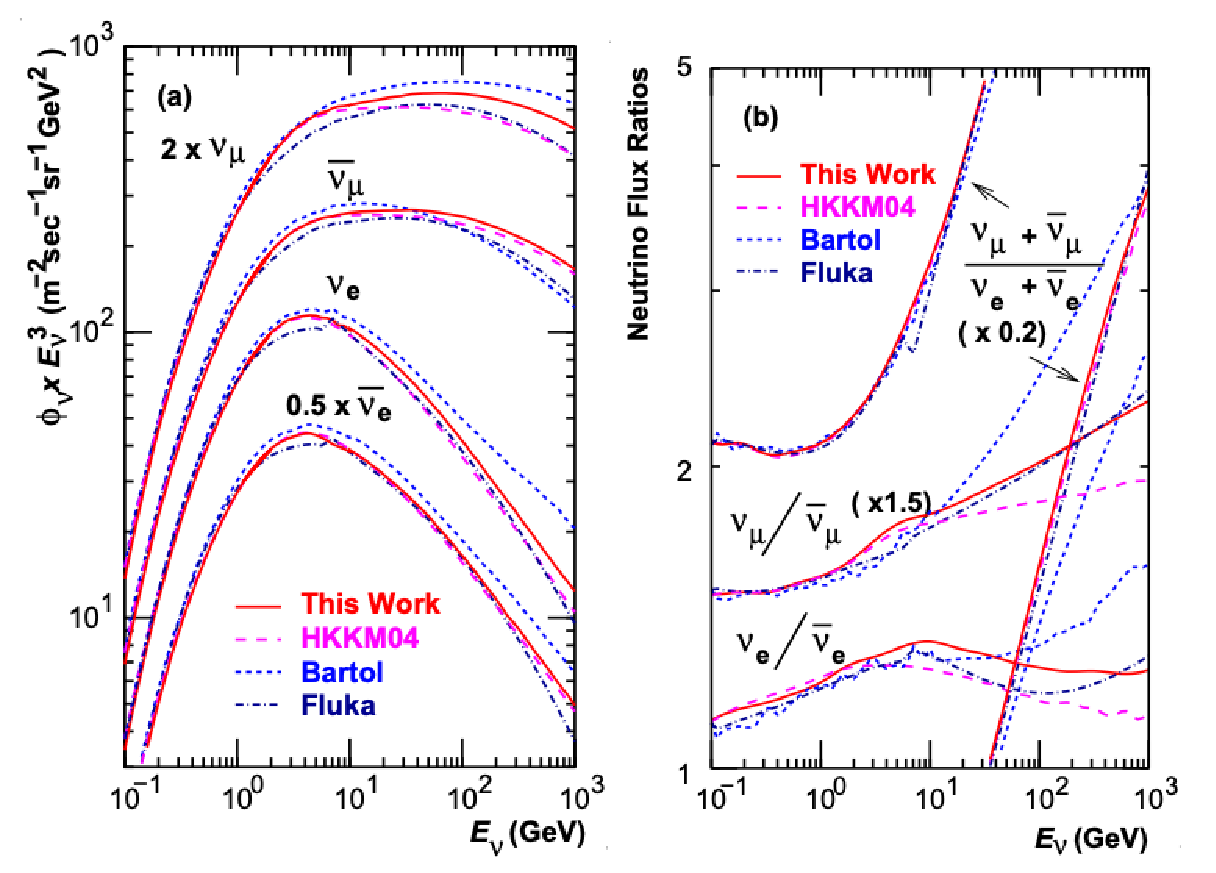
\includegraphics[width=\textwidth, trim={0mm 0mm 0mm 0mm}, clip,page=1]{Figures/Theory/AtmosphericNuFlux.pdf}
  \end{subfigure}
  \caption{Left panel: The atmospheric neutrino flux for different neutrino flavours as a function of neutrino energy which compares the 2007 Honda model (``This work'') \cite{Honda_2007}, the 2004 Honda model (``HKKM04'')\cite{PhysRevD.70.043008}, the Bartol model \cite{Barr_2004} and the FLUKA model. Right panel: indicates the ratio of the flux models between each model. Taken from \cite{Honda_2007}.}
  \label{fig:NeutrinoOscillationPhysics_AtmosphericNeutrinoFlux}
\end{figure}

The oscillations present in atmospheric neutrinos still follow the same \quickmath{L/E} probability presented in \autoref{sec:NeutrinoOscillationPhysics_3FlavourOsc}, but unlike a fixed beam experiment, the baseline for each neutrino is dependent upon the zenith angle with respect to Z-axis of the detector as illustrated by \autoref{fig:NeutrinoOscillationPhysics_ZenithAngle}. Neutrinos coming from interactions taking place in the atmospheric above the detector (\quickmath{\cos(\theta)=1.0}) only travel the height of the atmosphere before being observed within the detector; a distance of \quickmath{O(20)\text{km}}. However, neutrinos which are observed as coming from directly below the detector (\quickmath{\cos(\theta)=-1.0}) have travelled \quickmath{O(6 \times 10^{3})\text{km}} from interactions in the atmosphere on the opposite side of the Earth. As discussed in \autoref{sec:NeutrinoOscillationPhysics_MSW}, any neutrino passing through the Earth is subject to matter effects. These effects are most notable for any neutrino which passes through the Earth's core (\quickmath{\cos(\theta)<-0.45}).

\begin{figure}[h]
  \begin{subfigure}[t]{0.50\textwidth}
    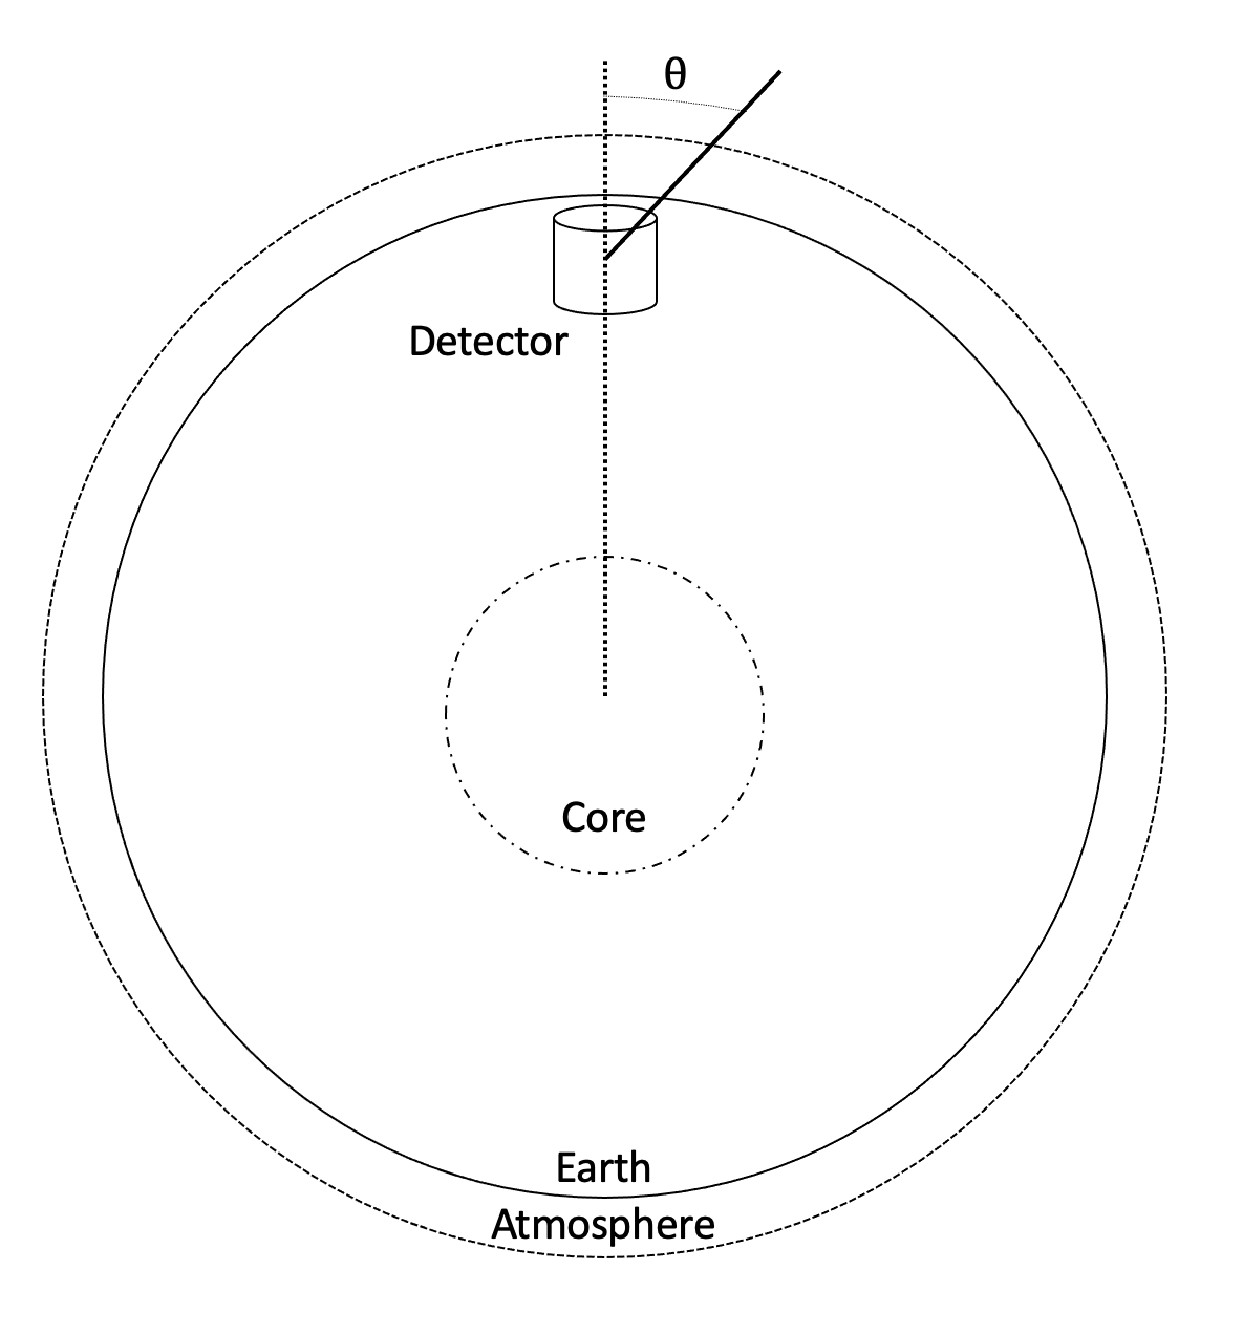
\includegraphics[width=\textwidth, trim={0mm 0mm 0mm 0mm}, clip,page=1]{Figures/Theory/ZenithAngle.pdf}
  \end{subfigure}
  \caption{A diagram illustrating the definition of zenith angle as used in the Super Kamiokande experiment \cite{Ashie_2005}.}
  \label{fig:NeutrinoOscillationPhysics_ZenithAngle}
\end{figure}

\autoref{fig:NeutrinoOscillationPhysics_NuFluxZenithAngleDep} highlights the neutrino flux as a function of zenith angle for different slices of neutrino energy. For medium to high energy neutrinos (and to a lesser degree for low energy neutrinos), the flux is approximately symmetric around \quickmath{\cos(\theta)=0}. To the accuracy of this approximation, the systematic uncertainties associated with atmospheric flux for comparing upward-going and down-going neutrino cancels. This allows the down-going events, which are mostly insensitive to oscillation probabilities due to the small \quickmath{L/E}, to act as a unoscillated prediction (similar to a near detector in an accelerator neutrino experiment).

\begin{figure}[h]
  \begin{subfigure}[t]{0.90\textwidth}
    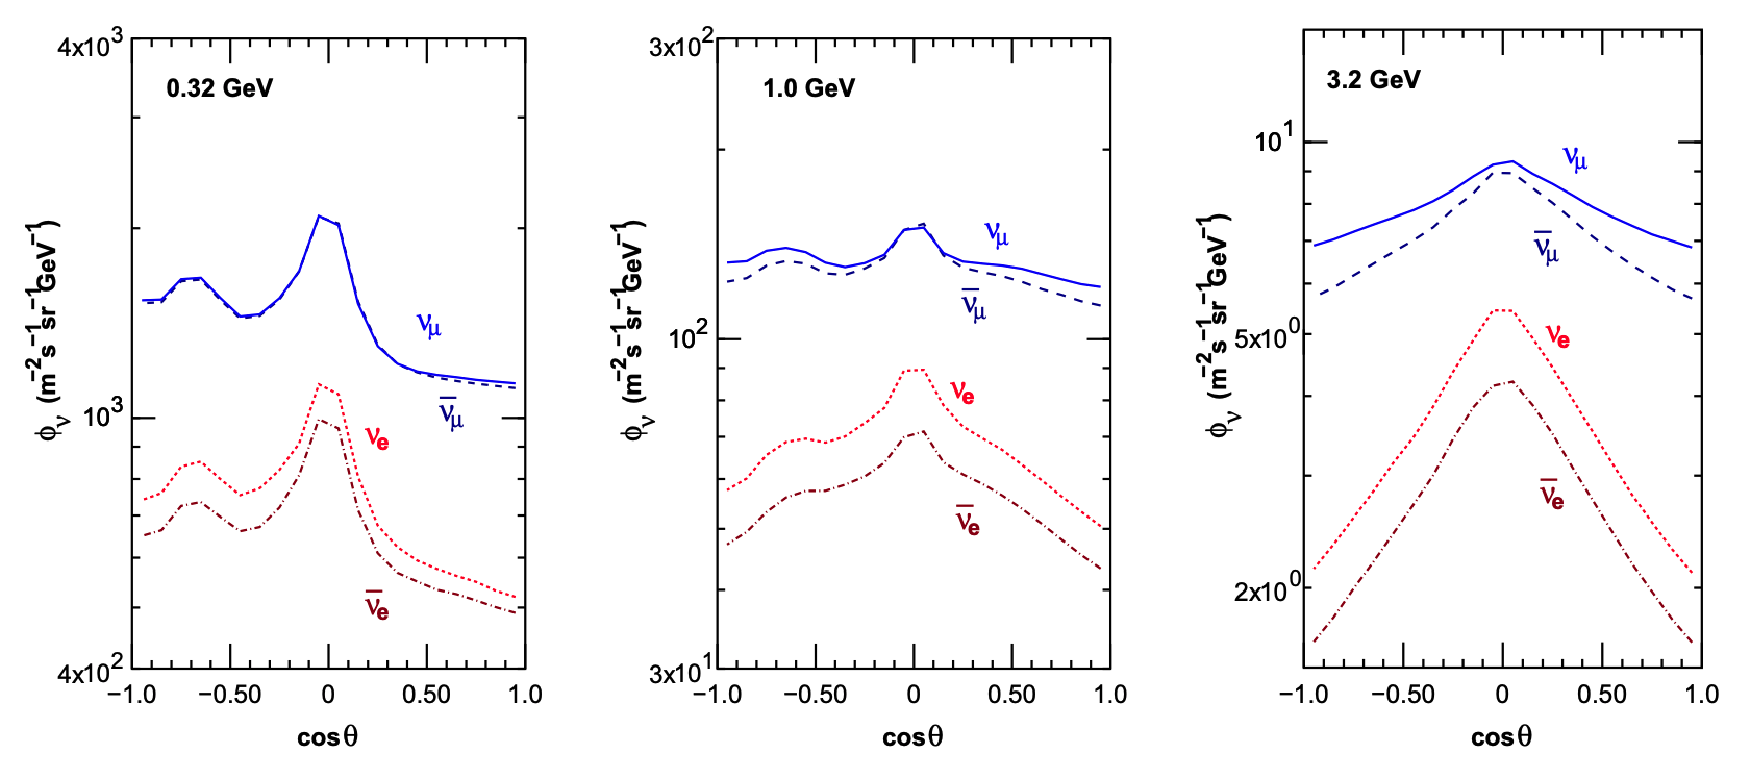
\includegraphics[width=\textwidth, trim={0mm 0mm 0mm 0mm}, clip,page=1]{Figures/Theory/NuFluxZenithAngleDep.pdf}
  \end{subfigure}
  \caption{Predictions of the summed neutrino and antineutrino flux for electron and muon neutrinos from the Bartol \cite{Barr_2004}, Honda \cite{Honda_2007} and FLUKA \cite{etde_20239111} models as a function of zenith angle with respect to the detector. Left panel: \quickmath{0.3 < E_{\nu} < 0.5}. Middle panel: \quickmath{0.9 < E_{\nu} < 1.5}. Right panel: \quickmath{3.0 < E_{\nu} < 5.0}. Taken from \cite{Ashie_2005}.}
  \label{fig:NeutrinoOscillationPhysics_NuFluxZenithAngleDep}
\end{figure}

Precursory hints of atmospheric neutrinos were observed in the mid-1960s searching for \quickmath{\overset{(-)}{\nu_\mu} + X \rightarrow X^{*} + \mu^{\pm}} \cite{Reines1965-cf}. These experiments were located in deep underground laboratories to reduce the cosmic muon background. These were replaced with the IMB-3 \cite{PhysRevLett.66.2561} and Kamiokande \cite{Hirata1992-qz} experiments which measured a deficit of muon neutrinos compared to electron neutrinos \quickmath{R(\nu_{\mu}/\nu_{e})}. Both experiments were found to have a consistent measurement, with \quickmath{R(\nu_{\mu}/\nu_{e}) = 0.67 \pm 0.17} and \quickmath{R(\nu_{\mu}/\nu_{e}) = 0.60 \substack{+ 0.07 \\ -0.06} \pm 0.05}. Soudan-2 \cite{Allison1997-qz} determined similar measurements. Super-Kamiokande (SK) \cite{Ashie_2005} extended this analysis by fitting oscillation parameters in \quickmath{\nu_\mu \rightarrow \nu_\tau} which found best fit parameters \quickmath{\sin^{2}(2\theta) > 0.92} and \quickmath{1.5 \times 10^{-3} < \Delta m^{2} < 3.4 \times 10^{-3} \text{eV}^{2}}.

Since then, atmopsheric neutrino exeperiments have begun making precision measurements of the \sinsqatm and \quickmath{|\Delta m^{2}_{32}|} oscillation parameters, and to a lesser extent the sign of \delmsqatm through the matter resonance present for any neutrinos passing through the Earth. Atmospheric neutrino oscillation is dominated by \quickmath{P(\nu_{\mu} \rightarrow \nu_{\tau})}, where SK observed a \quickmath{4.6\sigma} discovery of \quickmath{\nu_{\tau}} appearance \cite{Li_2018}. \autoref{fig:NeutrinoOscillationPhysics_AtmosphericParamContour} illustrates the current estimates on the atmospheric mixing parameters from a wide range of atmospheric and accelerator neutrino observatories.

\begin{figure}[h]
  \begin{subfigure}[t]{0.90\textwidth}
    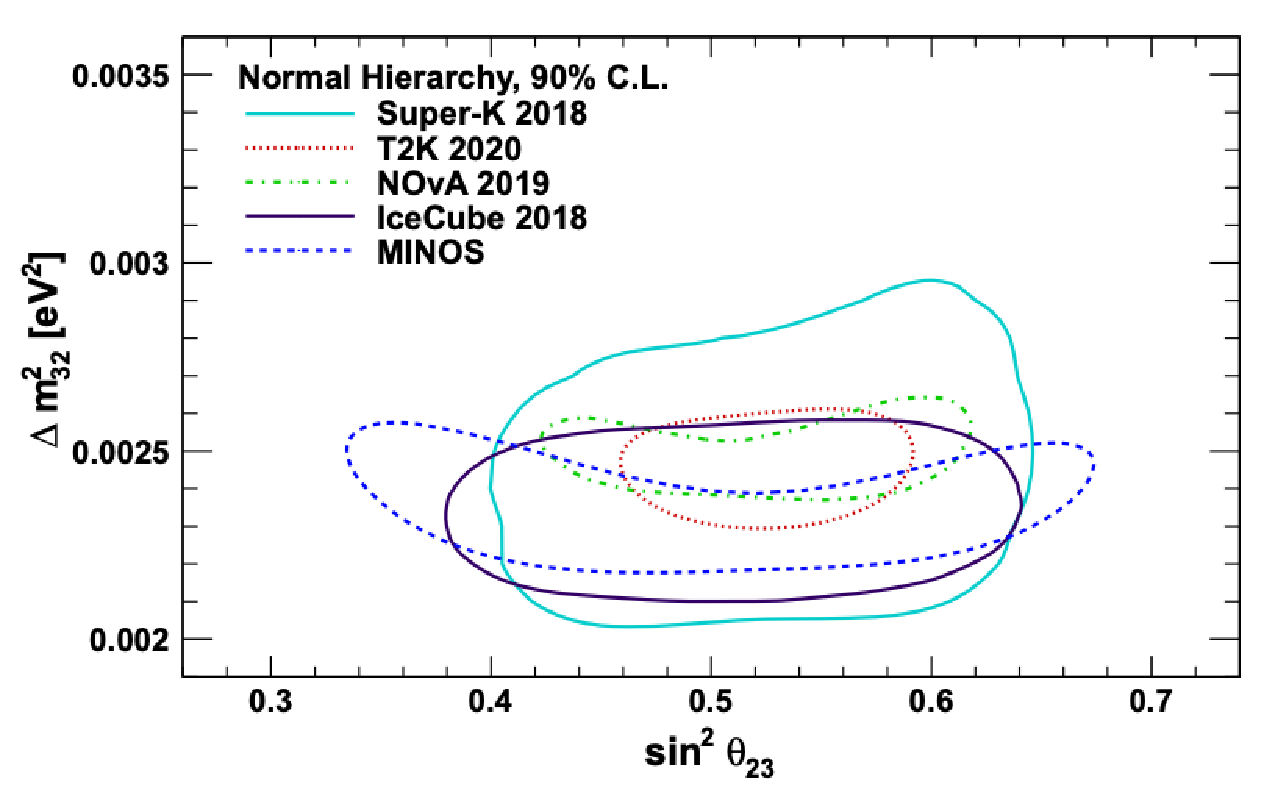
\includegraphics[width=\textwidth, trim={0mm 0mm 0mm 0mm}, clip,page=1]{Figures/Theory/AtmosphericParams.pdf}
  \end{subfigure}
  \caption{Constraints on the atmospheric oscillation parameters, \sinsqatm and \delmsqatm, from atmospheric and long baseline experiments SK \cite{Kamiokande_Collaboration2017-nf}, T2K \cite{T2K_Collaboration2018-sm}, \quickmath{\text{NO}\nu\text{A}} \cite{Acero2019-rw}, IceCube \cite{Aartsen2018-cz} and MINOS \cite{Adamson2014-tt}. Figure taken from \cite{Athar_2022}.}
  \label{fig:NeutrinoOscillationPhysics_AtmosphericParamContour}
\end{figure}

\subsection{Accelerator Neutrinos}
\label{subsec:NeutrinoOscillationPhysics_AcceleratorNeutrinos}

The concept of using a man-made source of neutrinos, a ``neutrino beam'',  was first realised in 1962 \cite{Danby1962-ph} and led to the first discovery that \quickmath{\nu_{e}} and \quickmath{\nu_{\mu}} were in fact different particles. Since then, many large scale experiments have followed which all using the same fundamental concepts. A proton beam is aimed at a target, producing charged mesons which then decay to neutrinos and the associated leptons. The mesons can be sign-selected by the use of magenetic focussing horns to generate a neutrino or antineutrino beam. Absorbing material and the rock between the target and detector absorb all particles barring the neutrinos. Pions are the primary meson which decay and depending on the orientation of the focussing, a predominately muon neutrino beam is generated via \quickmath{\pi^{+} \rightarrow \mu^{+} + \nu_{\mu}} or \quickmath{\pi^{-} \rightarrow \mu^{-} + \bar{\nu}_{\mu}}. Despite this, an approximately \quickmath{10\%} ``wrong-sign'' neutrino background of \quickmath{\nu_{e}} is generated via the decay of muons or kaons. 

As the inital proton beam can be tuned resulting in a tunable neutrino energy spectra, the advantage of these type of experiments is that they can be focused in on the oscillation dip presented by the \quickmath{L/E} term in \autoref{eq:NeutrinoOscillationPhysics_PMNS_2FlavourOscProb} using the two flavour approximation. This tuning means that accelerator experiments are typically more sensitive to the atmospheric mixing parameters. However, the disadvantage compared to atmospheric neutrino experiments is that the baseline (or length of the neutrino beam) has to be shorter due to the lower flux. Consequently, there is typically less sensitivity to matter effects and the ordering of the neutrino mass eigenstates.

A neutrino experiment measures

\begin{equation}
  \label{eq:NeutrinoOscillationPhysics_DetectorMeasurement}
  R(\vec{x}) = \Phi(E_{\nu}) \times \sigma(E_{\nu}) \times \epsilon(\vec{x}) \times P(\nu_{\alpha} \rightarrow \nu_{\beta}),
\end{equation}

where \quickmath{R(\vec{x})} is the event rate of neutrinos at position \quickmath{\vec{x}}, \quickmath{\Phi(E_{\nu})} is the flux of neutrinos with energy \quickmath{E_{\nu}}, \quickmath{\sigma(E_{\nu})} is the cross section of the interaction and \quickmath{\epsilon(\vec{x})} is the efficiency of the detector. Thus, in order to leverage the most out of an accelerator neutrino experiment, the flux and cross section systematics need to be constrained. This is typically done via the use of a ``near detector'', situated at a baseline of \quickmath{O(1)\text{km}} which observes the unoscillated neutrino flux and constrains the parameters used within the flux and cross section model.

Long baseline experiments became the forerunners of precision measurements of oscillation parameters. MINOS \cite{PhysRevLett.97.191801} and K2K \cite{PhysRevLett.9.36} confirmed the \quickmath{\nu_{\mu} \rightarrow \nu_{\mu}} oscillations seen in atmospsheric neutrino experiments by finding consistent mixing parameter values for \sinsqatm and \delmsqatm. The current generation of accelerator neutrino experiments, T2K and \NOVA extended this field by observing \quickmath{\bar{\nu}_{\mu} \rightarrow \bar{\nu}_{e}} and lead the sensitivity to atmospheric mixing parameters as seen in \autoref{fig:NeutrinoOscillationPhysics_AtmosphericParamContour} \cite{PhysRevLett.123.151803}. The two experiments differ in their peak neutrino energy, baseline and detection technique. The \NOVA experiment is situated at a baseline of \quickmath{810\text{km}} from the NuMI beamline which delivers \quickmath{2\text{GeV}} neutrinos whereas T2K neutrinos are peaked around \quickmath{0.6 \text{GeV}} and propagate \quickmath{295\text{km}}. The \NOVA experiment also uses functionally identical detectors (near and far) which allows the approximately cancellation of detector systematics whereas T2K uses a plastic scintillator technique at the near detector and a water Cherenkov far detector. The future generation experiments DUNE \cite{Abi2020-cm} and Hyper-Kamiokande \cite{Hyper-Kamiokande_Proto-Collaboration2015-ac} will succeed these experiments as the high precision-era of neutrino oscillation parameter measurements develops.

Several anomalous results have been observed in the LSND \cite{PhysRevD.64.112007} and MiniBooNE \cite{PhysRevLett.110.161801} detectors which were designed with purposefully short baselines. Parts of the neutrino community attributed these results to be oscillations induced by a fourth ``sterile'' neutrino \cite{Blanco_2020} but several searches in other experiments, MicroBooNE \cite{10.48550/arxiv.2110.14054} and KARMEN \cite{PhysRevD.65.112001} found no hints of additional neutrino species. 

\subsection{Reactor Neutrinos}
\label{subsec:NeutrinoOscillationPhysics_ReactorNeutrinos}

As illustrated in the first discovery of neutrinos (\autoref{sec:NeutrinoOscillationPhysics_Discovery}), nuclear reactors are a very powerful man-made source of electron antineutrinos. For reactors which use low-enriched uranium \quickmath{^{235}\text{U}} as fuel, the antineutrino flux is dominanted by the \quickmath{\beta}-decay fisson of \quickmath{^{235}\text{U}}, \quickmath{^{238}\text{U}}, \quickmath{^{239}\text{Pu}} and \quickmath{^{241}\text{Pu}} \cite{Kim2013-ye} as illustrated in \autoref{fig:NeutrinoOscillationPhysics_ReactorNeutrinoProduction}.

\begin{figure}[h]
  \begin{subfigure}[t]{0.90\textwidth}
    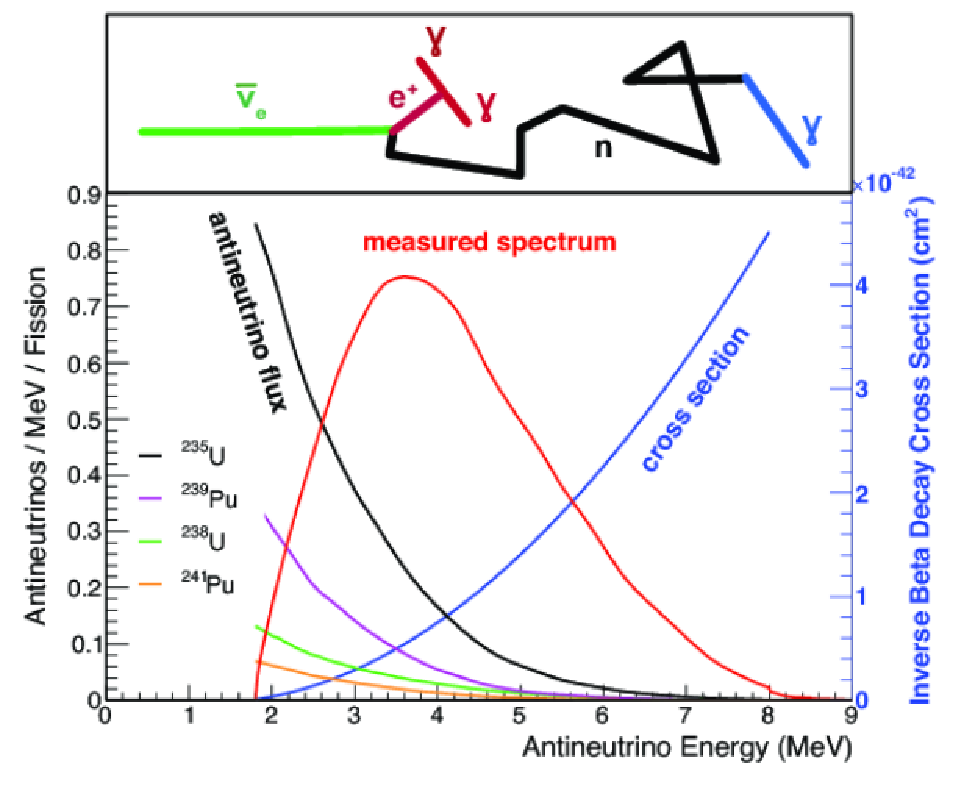
\includegraphics[width=\textwidth, trim={0mm 0mm 0mm 0mm}, clip,page=1]{Figures/Theory/ReactorNeutrinoProduction.pdf}
  \end{subfigure}
  \caption{Reactor electron antineutrino fluxes for \quickmath{^{235}\text{U}} (Black), \quickmath{^{238}\text{U}} (Green), \quickmath{^{239}\text{Pu}} (Purple) and \quickmath{^{241}\text{Pu}} (Orange) isotopes. The inverse \quickmath{\beta}-decay cross section is given in Blue and corresponding measurable neutrino spectrum is highlighted in Red. Top panel: Schematic of Inverse \quickmath{\beta}-decay interaction. Taken from \cite{SajjadAthar:2021prg}.}
  \label{fig:NeutrinoOscillationPhysics_ReactorNeutrinoProduction}
\end{figure}

Due to their low energy, reactor electron antineutrinos interact via the inverse \quickmath{\beta}-decay (IBD) interaction. The typical signature contains two signals delayed by \quickmath{O(200)\mu\text{s}}; firstly the prompt photons from positron annihilation, and secondly the photons emitted (\quickmath{E_{tot}^{\gamma} = 2.2\text{MeV}}) from de-excitation after neutron capture on hydrogen. Recently, SK included gadolinium dopanants into the ultra-pure water to increase the energy released from the photon cascade to \quickmath{\sim 8\text{MeV}} and reduce the time of the delayed signal to \quickmath{\sim 28 \mu \text{s}}. This improves the detector's ability to distinguish between background and signal events \cite{Abe2022-ij}.

There are many short baseline experiments (\quickmath{\text{L} \sim O(1)\text{km}}) which have measured the \sinsqreac and \delmsqatm oscillation parameters. Daya Bay \cite{PhysRevLett.108.171803}, RENO \cite{PhysRevLett.108.191802} and Double Chooz \cite{PhysRevLett.108.131801} have all provided precise measurements, with the first discovery of a non-zero \quickmath{\theta_{13}} made by Daya Bay and RENO. The constraints on \sinsqreac by the reactor experiments lead the field and are often used as external inputs to accelerator neutrino experiments to improve their sensitivity to \dcp and mass hierarchy determination. One curiosity of these short baseline reactor experiments is the `\quickmath{5 \text{MeV}} excess' \cite{Berryman_2019}. First observed in 2014 \cite{For_the_RENO_Collaboration2015-zy, Abe_2014}, all three experiments listed observed a shape excess in events around \quickmath{E_{\nu} \sim 5 \text{MeV}}. The reason behind this excess is speculated to be either oscillations to sterile neutrinos or a fault in the Huber-Mueller model \cite{Mueller_2011}. At this time, the latter is favoured as Daya Bay \cite{PhysRevLett.123.111801} observed substantial evidence (\quickmath{4.0\sigma}) of correlation between the excess and the \quickmath{^{235}\text{U}} electron antineutrino flux.
%Other neutrino experiments, PROSPECT \cite{PhysRevD.103.032001} and STEREO \cite{STEREO} show similar results data to help determine the cause of the excess.
JUNO-TAO \cite{junocollaboration2020tao}, a small collaboration within the larger JUNO experiment, is a next generation reactor experiment which aims to precisely measure the isotopic antineutrino yields from the different fission chains. Alongside this, it aims to explain the `\quickmath{5 \text{MeV}} excess' by conducting a search for sterile neutrinos with a mass scale of around \quickmath{1 \text{eV}}.

Kamland \cite{Decowski2016-hh} is the only experiment to have observed reactor neutrinos using a long baseline (flux weighted averaged baseline of \quickmath{L \sim 180\text{km}}) which allows it to have sensitivity to \delmsqsol. Combined with the SK solar neutrino experiment, the combined analysis puts the most stringent constraint on \delmsqsol \cite{PhysRevD.83.052002} which is used as a prior uncertainty with accelerator neutrino experiments.

\section{Measurement Summary}
\label{sec:NeutrinoOscillationPhysics_MeasurementSummary}
